%# -*- coding: utf-8-unix -*-
%%==================================================
%% chapter5.tex for SJTU Master Thesis
%%==================================================

%\bibliographystyle{sjtu2}%[此处用于每章都生产参考文献]
\chapter{查询系统的分布式部署}
\label{chap:c5}

完成了前面几章叙述的内容后,搜索平台经过测试后就已经可以正式上线了。然而在系统实际运行的过程中,却发现系统有一些因为只有单台服务器而产生的问题。例如:
\begin{enumerate}
\item 当服务器负荷较大,如正在运行其它高系统占用率服务时,平台的搜索速度会有极大地减缓。
\item 当查询平台的进程因内存溢出等原因崩溃或服务器计算机重启时,网站的搜索结果会直接报错。
\end{enumerate}

这些实际问题的产生也体现了搜索平台对分布式服务器的需求。对于大规模的查询系统,单台服务器往往有它显而易见的局限性,例如负载上限较低,稳定性较差,容错性低等。使用多台服务器部署分布式云架构搜索平台,是解决单台服务器局限性的一种很好的方式。这种架构有如下优点:
\begin{enumerate}
\item 实现了多台服务器查询时的负载均衡,使搜索服务器可以动态分配计算资源,达到性能最大化;
\item 实现了多台服务器上配置文件的集中管理,将多台服务器的配置文件统一挂在在一个节点上,避免了多份配置文件管理上的不便;
\item 实现了多台服务器运行状态的统一监管,在任意节点上可以查看所有节点的运行状态;
\item 采用了分布式的自组织架构,并没有严格意义上的主服务器,任何一个服务器挂掉,都不会影响到整个系统的正常运行;
\item 实现了服务进程的自动恢复,当任何一台电脑需要重启或关闭服务进程时,直接关闭该进程不会中断搜索服务的提供,并且在服务进程重新启动后,进程能自动恢复到云上;
\item 实现了索引文件的备份。对于索引文件的每一个分片,其备份数目都与云平台上节点数目相同,这在保证了系统容忍任意(N-1)个节点同时故障的同时,也对索引文件实现了多次备份,避免了某几个服务器硬盘损坏导致的数据不可恢复地丢失。
\end{enumerate}

当然,要实现拥有这么多功能的云架构搜索平台,就不可避免地需要大大增加整个系统的复杂度。虽然目前互联网上有一些相关的资料,但是大部分资料都是让分布式服务运行不报错就浅尝辄止,而几乎没有资料讲述了完整地实现一个功能完整的分布式搜索服务器的方法。因此在做这一部分工作的时间里,我付出了大量的时间去摸索实现分布式服务的各个环节,也花费了比预期更长的时间才完成了分布式搜索平台的所有功能。

实现分布式搜索平台的第一步就是要设计系统的架构。架构设计的目的是要在尽量不改动之前实现的功能模块的基础上为系统引入分布式的服务,同时要使分布式的系统尽可能地稳定,功能强大,并且易于维护。

\section{分布式系统的架构}

要想实现搜索平台的分布式部署,就必须引入分布式程序的协调工具。在本平台中,我们使用Apache Zookeeper来进行分布式服务的协调。Zookeeper在本应用中,显式地可以完成配置文件云节点的挂载以实现配置文件的统一管理,隐式地可以完成主服务器选举、负载均衡、同步数据、锁死避免等分布式服务所需要的功能。经过初步设计后,分布式平台的架构设计如下:
\begin{figure}[!htp]
  \centering
  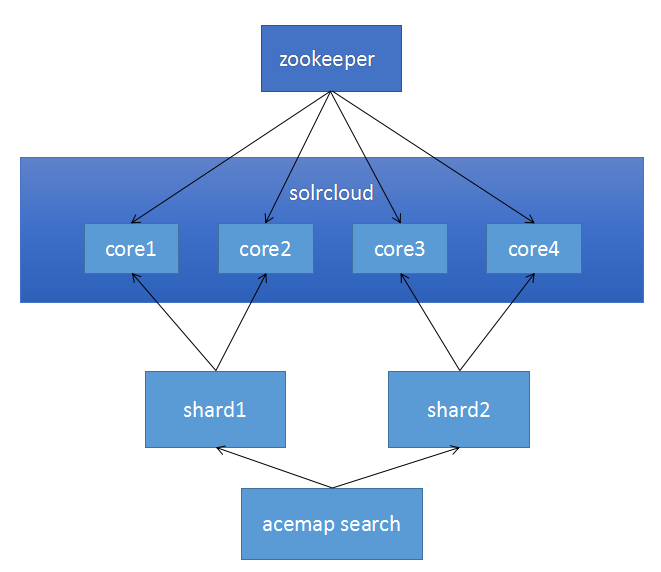
\includegraphics[width=0.6\textwidth]{zookeeper.png}
  \bicaption[fig:solrcloud]{云服务器初始架构}{云服务器初始架构}{Fig.}{Solrcloud Simplified}
\end{figure}

在这里,我们把原来单一的Solr实例(Instance,又叫Core)分为四个节点,并由一个Zookeeper服务器进行统一管理。同时,我们原本的单一索引文件被分成了两个片(Shard),每一个片分为两个相同的备份。这样一来,每个Solr节点里恰保存一份索引,并负责与该份索引相关的索引工作。我们将Core1与Core3放在同一台服务器上,Core2个Core4放在另一台服务器上,四台服务器上的两片索引文件和两片备份索引文件共同组成了索引集合(Collection)。

由于在实例中保存的配置文件难以同步修改,因此在这四个Solr实例中均不保存任何配置文件,所有的配置文件我们统一保存在Zookeeper的数据节点中。在索引构建的阶段,四个实例分别读取Zookeeper数据节点中的配置文件,确定自己的索引结构,并由Zookeeper内部算法决定将每一篇文档转发到哪个分片中进行索引;在查询阶段,Zookeeper决定将查询请求分配给哪些较为空闲的节点,并通过配置文件决定给Solr实例的查询请求格式,由选举出的主实例(Leader)进行结果整合与发布。

当四个节点中的任意一个节点因为意外(例如索引文件损坏,进程意外终止等)无法正常工作时,Zookeeper会自动检测到节点的异常,并将其标记为宕机(Down)状态或离线(Gone)状态,此时整个系统的服务并不会终止,而是会由剩下的节点分配承担所有任务。由于目前架构中任意一台服务器上都保存着一份所有索引的备份,所以只要不是所有的计算机服务器全部宕机,完整的服务功能都会保持。当意外关闭的节点被重新注册回Zookeeper时,Zookeeper会尝试恢复该节点并使其回复正常工作。

以上的架构看似很完美,然而仍然存在一个严重的缺陷——那就是Zookeeper节点的单一性会导致其反而成为系统鲁棒性的短板。换句话说,虽然对于目前的架构任意Solr节点的宕机都不会造成服务故障,但是一旦Zookeeper服务本身出现故障,所有的服务都会跟着瘫痪。解决这一问题的方法有两个,一是将Zookeeper服务运行在几乎不需要维护重启的专门服务器上,二是针对Zookeeper服务器本身建立一个分布式架构。用通俗的话说,第二种解决问题的方法,就是用Zookeeper Cloud来管理Solr Cloud。该改进的架构如下图所示:
\begin{figure}[!htp]
  \centering
  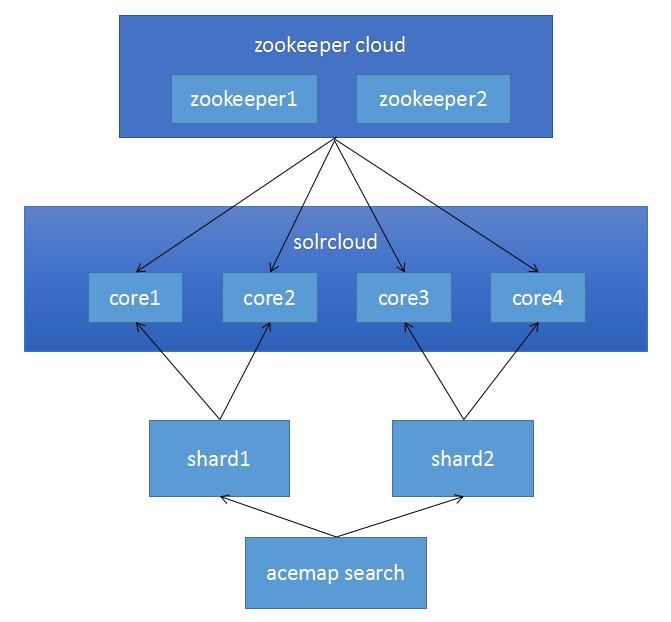
\includegraphics[width=0.6\textwidth]{zookeepercloud.png}
  \bicaption[fig:solrcloudadv]{云服务器改进架构}{云服务器改进架构}{Fig.}{Solrcloud Advanced}
\end{figure}
此时,Zookeeper不仅管理着四个Solr节点,同时也管理着两个Zookeeper节点。与Solr节点自动选取Leader类似,Zookeeper节点的Leader也是由内部自动选举得到的。两个Zookeeper节点的存在分担了Zookeeper服务器宕机的风险,使得其中任何一个Zookeeper服务器故障都不会影响到系统整体的正常工作。一个显而易见的好处是,在这个架构下我们可以只配置两台服务器计算机,并在每台计算机上部署一个Zookeeper节点和两个Solr节点,此时任何一台计算机的重启都不会终止服务的正常提供。而如果不配置两个Zookeeper节点,运行着Zookeeper服务的计算机是不能重启的,否则整个服务就会崩溃。

但是这个方案和第一套方案相比也不是十全十美的。第一套解决方案能保证系统在上线后,能够用一套十分简单的流程来维护系统的所有功能,而对于第二套解决方案架构的系统,其维护过程会比第一套解决方案复杂很多,在非专业人士操作维护时可能会让服务器产生更多的故障。因此这里只是在理论上说明了第二套流程的可行性及其优势,在实际搜索平台的实现中,我们并没有采用云架构部署Zookeeper本身。

\section{分布式系统的部署}
这一部分介绍云服务器初始架构的部署方式。具体的部署命令可以参见附录1中,上面有详细的罗列。

首先,我们需要配置并启动一个Zookeeper服务。Zookeeper服务的配置需要指定5个参数,我们通过修改zoo.cfg文件以完成此处的配置。
\begin{enumerate}
\item tickTime:一次同步的时间周期,此处设置为2000ms;
\item initLimit:第一次同步过程花费时间周期数的限制,此处设置为10;
\item syncLimit:一次同步过程的时间周期数限制,即发送请求与得到相应之间的最大周期数间隔,此处设置为5;
\item dataDir:存放快照数据的目录,根据需要设置;
\item clientPort:服务运行的端口,所有的Solr节点都要通过这个端口注册到Zookeeper。
\end{enumerate}

配置好这些参数后,我们就可以启动Zookeeper服务了。启动Zookeeper服务后,我们可以打开其客户端(Client)查看内部文件情况,由于是新挂载的节点,所以里面是没有任何文件的。针对之后需要挂载的Solr服务,需要在Zookeeper上挂载一个空节点,这里起名为acemap节点。

接下来要将Solr服务器注册到Zookeeper上。我们在两台服务器上各启动一个Solr服务,然后在每一个Solr服务上运行两个实例节点。在这一过程中,首先需要配置Solr服务的host地址,由于本平台中两台服务器并不在同一个内网上,所以我们使用公网地址作为服务的Solr地址。然后,我们需要指定服务以云模式启动并挂在到Zookeeper的acemap节点上,并指定为其Java虚拟机分配的内存。

第一台服务器上的Solr服务启动后,Zookeeper的acemap节点上会自动保存一些基本的配置文件,打开其中的live\_nodes文件夹,可以看到对应与启动服务host名称的记录文件。启动第二台服务器上的Solr服务后,live\_nodes文件夹里会显示两个服务各自的记录文件。

之后,我们需要在两个Solr服务组成的集群上创建一个新的索引集合(Collection),并以2的冗余度创建两个分片。此时,这四个分片会被自动分配到四个Solr节点中,同时每台服务器上的Solr服务都会自动分配到两个不同的分片。

最后,我们需要实现配置文件的统一管理功能。这一功能可以借助zkcli.sh进行实现。我们先将所有的配置文件统一放入文件夹中,用zkcli.sh的upconfig方法可以将本地的文件夹传入Zookeeper对应节点上,downconfig方法可以将Zookeeper节点上的文件下载到本地。在文件夹被挂载到节点上之后,我们可以用linkconfig函数将节点与Solr云中的collection对应起来。

至此,Solr服务器的分布式部署已经基本完成,我们可以通过访问任何一个Solr服务器来管理这个分布式的集合(collection)。

\section{分布式系统的配置}
分布式系统的配置方法和单台服务器的配置方法大同小异。在集合整体的视角下,四个子节点组成的整体可以视作一个大的单台服务器,因此,系统配置的过程和单台服务器一样,需要先配置solrconfig.xml文件,再进行索引结构设计与文档导入,最后进行查询指令的设计。不同的是,在配置文件与索引结构设计完成后,注意需要用reload指令确保指令被同步到了每个节点之中。

此外,由于索引被分成了两个独立的片,因此查询指令中新增了一条\&shard=XXX的命令,用以只在某个片中搜索结果。更进一步地,可以指定只在某个shard的某个特定的备份中进行查询。这种查询方式称作分布式查询。(参考资料https://cwiki.apache.org/confluence/display/solr/Distributed+Requests)

既然Solr云架构拥有分布式查询的功能,那就说明shard的构建过程除了交给系统自动进行外,也可以人为地进一步自定义。例如,在集合创建时,可以用router.name属性在决定每一条文档被分发到哪一个具体的片上。例如对于本学术网站的搜索平台,router.name可以由论文属于计算机领域或是非计算机领域决定,通过将计算机领域的论文索引到其中一个片,非计算机领域的论文索引到另一个片,就可以用分布式查询的方法高效的在计算机或非计算机论文这两个子集中分别查询论文。但是由于实际上非计算机领域和计算机领域论文这一划分方式并不均匀,前者的数量实际上会远远多于后者,所以会导致资源分配不均匀的问题。我们可以通过添加服务器,并利用片分割(Shard Splitting)的方法将较大的片进一步分割存储到更多的服务器中,以达到负载均衡。